\documentclass[a4paper,11pt]{article}
\usepackage[utf8x]{inputenc}
\usepackage{fancyhdr}
\usepackage{graphics}
\usepackage{amsmath}    % need for subequations
\usepackage{graphicx}   % need for figures
\usepackage{verbatim}   % useful for program listings
\usepackage{color}      % use if color is used in text
\usepackage{subfigure}  % use for side-by-side figures
\usepackage{hyperref}   % use for hypertext links, including those to external

\pagestyle{fancy}

\lhead[\thepage]{Grupo Número 2}      % Note the different brackets!
\rhead[Grupo Número 2]{Julio 2010}

%opening
\title{Trabajo Práctico Final}
\author{Guillermo Campelo\\Juan Ignacio Goñi\\Juan
Tenaillon\\Santiago Vazquez}

\begin{document}

\maketitle

\begin{abstract}
El siguiente informe describe cómo se diseñó e implementó el \textbf{Rally
Uribe
100K}. 
Mediante el uso de imágenes se describe cómo fueron diseñadas e implementadas
las distintas partes que componen al total de la aplicación.  También se
presentan los inconvenientes que surgieron a lo largo del desarrollo y cómo el
equipo decidió solucionarlos.  Por último se explicará cómo se utiliza el
juego,
cómo se modifican las distintas opciones de configuración del mismo y las
conclusiones.
\end{abstract}

\section{Introducción}

Haciendo uso del Framework JMonkey, se diseñó y desarrolló un juego de rally,
llamado Rally Uribe 100K.  A continuación, se describe cómo fue realizado el
mismo, qué características posee y la forma en que se utiliza el mismo.

Para el diseño e implementación del juego, partimos de la base del ejemplo
proporcionado por el Framework utilizado, y tomando esa base, se realizó
el desarrollo de las nuevas características.

En la sección \ref{el_juego} se explicará cómo es el juego, los distintos
estados del mismo, cómo es el sistema de puntaje y los sonidos del mismo.

En la sección \ref{caracteristicas} se explicará qué características
adicionales fueron desarrolladas para el juego, como las texturas procedurales,
los screenshots, los arbustos billboard, los skybox intercambiables y demás
características del mismo.

En la sección \ref{mododeuso} se explicará cómo se utiliza el juego,
explicando
las teclas a utilizar por defecto, además de explicar cómo utilizar las
distintas opciones del menú.

En la sección \ref{configuracion} se mostrarán las distintas opciones de
configuración, así como los valores recomendados para la misma.  También se
explicará cómo definir nuevas pistas, para que el usuario del mismo pueda
crear
sus propios recorridos y utilizarlos con el juego.

Por último, en la sección \ref{conclusiones} se presentarán las conclusiones
alcanzadas por el equipo, además de posibles extensiones al mismo y la
enseñanza obtenida del diseño y desarrollo del mismo.

\section{El Juego}
\label{el_juego}

En esta sección se explicará el juego en sí.  El objetivo del mismo, el modo
de
juego, los distintos estados, cómo es el sistema de puntajes y los sonidos
utilizados en el mismo.

\subsection{Descripción}
El juego consiste en recorrer una pista de carreras, ambientada como si fuera
de Rally.  El ambiente en el cual se mueve el auto, está compuesto de un
terreno, con una pista delimitada, con un conjunto de objetos que la componen.

El objetivo del mismo, es dar tres vueltas al recorrido propuesto.  Además de
completar la totalidad de las vueltas, el jugador debe transitar por la
totalidad de los checkpoints, en el orden determinado por la pista.  En caso de
saltearse uno el juego no le permitirá transitar exitosamente por los
siguientes, y el jugador deberá volver hacia atrás y transitar por el
checkpoint adeudado.

Al finalizar las tres vueltas, el jugador recibirá el tiempo de su recorrido, y
mientras más bajo sea ese tiempo, más chances tendrá de ingresar al listado
de
los puntajes más altos.
\subsection{Modo de Juego}
Hay un solo modo de juego, y este consiste en intentar realizar el menor tiempo
posible en la realización de las tres vueltas a la pista.
\subsection{Estados del Juego}
Hay tres estados diferenciados en el juego.  Antes de comenzar a jugar, durante
el juego y luego de jugar.

Antes de comenzar a jugar, el jugador encuentra el menú principal de la
aplicación, el cual le presenta todas las opciones disponibles.  Una vez que el
usuario selecciona la opción para comenzar a jugar, se realiza la transición
al
siguiente estado, el juego en sí.

\begin{figure}
\begin{minipage}[b]{0.5\linewidth}
\centering
 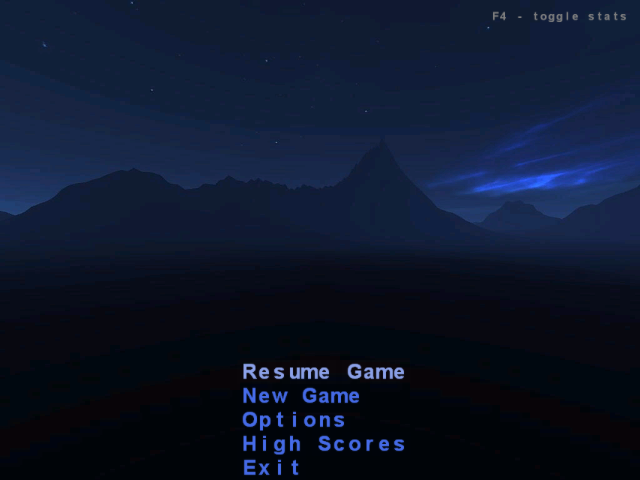
\includegraphics[scale=0.250]{./main_menu.png}
 % startinggrid.png: 640x480 pixel, 72dpi, 22.58x16.93 cm, bb=0 0 640 480
 \caption{Menú Principal.}
\label{fig:figure0}
\end{minipage}
\hspace{0.5cm}
\begin{minipage}[b]{0.5\linewidth}
\centering
 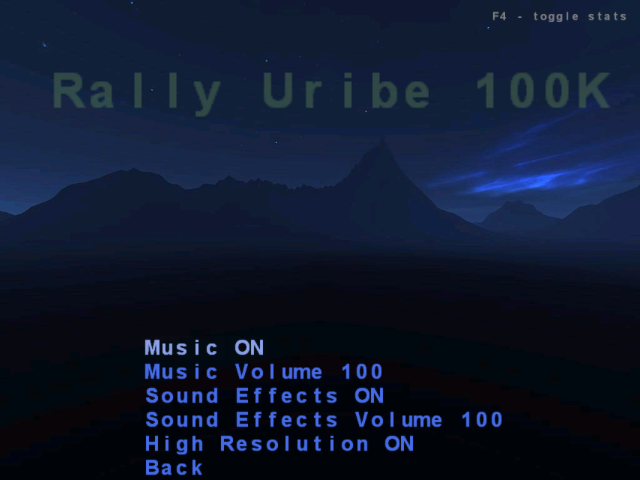
\includegraphics[scale=0.250]{./options_menu.png}
 % startinggrid.png: 640x480 pixel, 72dpi, 22.58x16.93 cm, bb=0 0 640 480
 \caption{Menú de Opciones.}
\label{fig:figure00}
\end{minipage}
\end{figure}

En este estado, es cuando el jugador maneja el vehículo a través del camino
propuesto.  El vehículo en esta ocasión, puede colisionar contra los distintos
objetos que componen la escena, como los árboles, los límites del terreno y
las
pirámides presentes en el recorrido.  Una vez finalizado el recorrido, se
realiza la transición al tercer y último estado del juego.

En este tercer y último estado, al usuario se le presenta el menú nuevamente,
donde podrá ver los puntajes máximos hasta el momento o comenzar nuevamente el
juego para tratar de mejorar su tiempo.

\subsection{Puntajes}
El juego tiene la opción de ver quienes fueron los jugadores que realizaron los
diez mejores tiempo en el recorrido a la pista.

Una vez finalizado el recorrido, se le presentará al jugador su tiempo total de
recorrido, y si el tiempo es lo suficientemente bueno, deberá ingresar su
nombre para comenzar a figurar en el listado de los mejores tiempos.

En el menú inicial del juego, el jugador puede elegir la opción de highscores,
para ver cuales son los mejores tiempos a la pista y quien fue el jugador que
los hizo.
\subsection{Sonidos}
El juego, como todos los de su tipo, tiene diferentes sonidos que ayudan a
ambientar el mismo.

Comenzando por los sonidos de ambiente, donde se decidió que se iban a utilizar
dos pistas para tener cierto cambio en la música de ambiente pero sin entrar en
la exageración de utilizar muchas pistas.

También fueron utilizados dos sonidos para ser utilizados por el vehículo para
denotar situaciones en las que se está acelerando y situaciones en las que no.

Por �ltimo, fue utilizado un sonido para los momentos en que el vehículo
colisiona contra algun objeto presente en el terreno.

Todos los sonidos propios del vehículo y su entorno fueron obtenidos de
Internet, de páginas de uso libre y gratuito.  Los temas utilizados para la
música ambiental, corresponden a la autoría de Santiago Vazquez, integrante
del
equipo.

\begin{figure}
\begin{minipage}[b]{0.5\linewidth}
\centering
 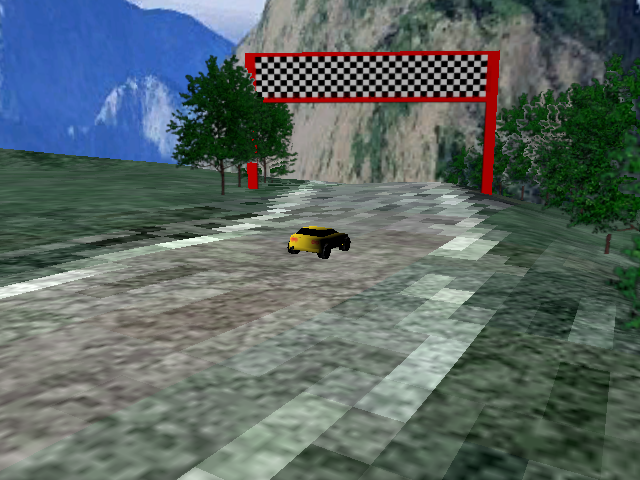
\includegraphics[scale=0.250]{./startinggrid.png}
 % startinggrid.png: 640x480 pixel, 72dpi, 22.58x16.93 cm, bb=0 0 640 480
 \caption{Grilla de Partida del Rally Uribe 100K. Bajo nivel de detalle.}
\label{fig:figure1}
\end{minipage}
\hspace{0.5cm}
\begin{minipage}[b]{0.5\linewidth}
\centering
 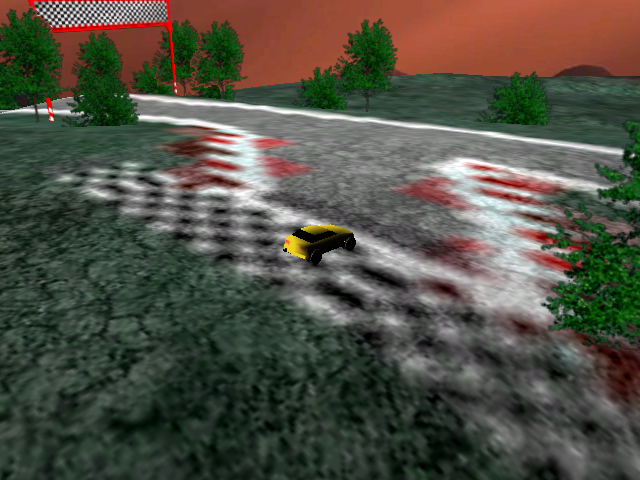
\includegraphics[scale=0.250]{./startinggrid_high.png}
 % startinggrid.png: 640x480 pixel, 72dpi, 22.58x16.93 cm, bb=0 0 640 480
 \caption{Grilla de Partida del Rally Uribe 100K. Alto nivel de detalle.}
\label{fig:figure2}
\end{minipage}
\end{figure}

\subsection{Iluminaci\'on}

El terreno en el cual se desarrolla el juego, cuenta con tres tipos distintos de
iluminaci\'on, una luz ambiente, una luz direccional y cinco luces puntuales que
iluminan la totalidad del recorrido.

La iluminaci\'on ambiente, est\'a configurada por defecto para tener un nivel
bajo de iluminaci\'on.  Se eligi\'o esto para que el resto de las luces tomen un
papel m\'as importante en la iluminaci\'on del escenario.

Los valores de rojo, verde, azul y canal alfa que determinan la intensidad y
color de la luz, son f\'acilmente configurables en el archivo
``global.properties'', bajo el elemento $TRACK1.AMBIENT.LIGHT$.

La luz direccional, est\'a configurada por defecto con un color rojo intenso y
est\'a emplazada encima del primer checkpoint del recorrido. La raz\'on de esta
decisi\'on radica en que ten\'iamos que buscar un lugar donde la luz fue
visible para demostrar la existencia de la misma, es por eso que cada vez que
el auto transita por debajo de la grilla de partida, se puede ver un color
rojizo en el techo del mismo.

Esta luz es tambi\'en configurable en cuanto a los colores rojo, verde, azul y
el canal alfa.  Para configurar esto, es necesario modificar en el archivo de
configuraci\'on, las propiedades que se encuentran bajo el elemento
$TRACK1.LIGHT.SPOTLIGHT$.

Por \'ultimo, las luces puntuales.  Las cinco luces puntuales est\'an en
distintos lugares a lo largo del recorrido.  A diferencia de los otros dos
tipos de iluminac\'on, estos tienen una posici\'on determinada por el usuario y
est\'an configuradas para dar una luz blanca.

Tanto la posici\'on de la luz como el color, son configurables.  Al igual que
el resto de las luces, para cambiar la posici\'on y color de estas, hay que
modificar las propiedades de cada luz en el archivo de configuraci\'on.  Cada
luz puntual est\'a contemplada bajo la propiedad $TRACK1.POINTLIGHTn$ donde $n$
es el n\'umero de la luz.

En las figuras \ref{fig:sinluz} y \ref{fig:conluz} se puede apreciar el juego
con las luces puntuales deshabilitadas y con las luces puntuales habilitadas
respectivamente.  Cabe destacar que en la figura \ref{fig:sinluz} puede
apreciarse una luz ambiental muy tenue junto con la luz direccional en color
rojo apuntando hacia abajo sobre el primer checkpoint.

\begin{figure}
\begin{minipage}[b]{0.5\linewidth}
\centering
 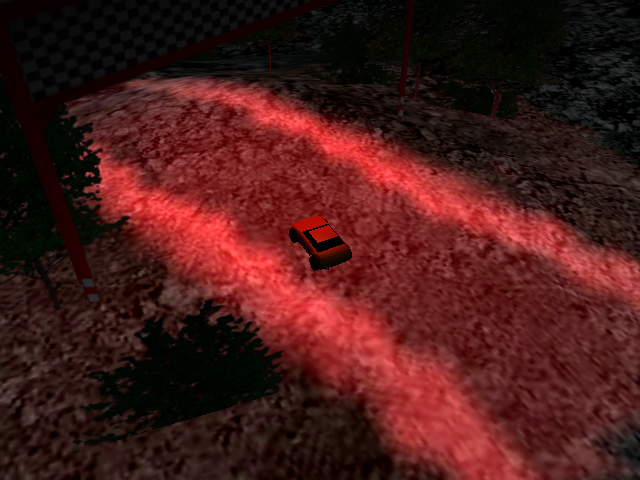
\includegraphics[scale=0.250]{./sinluz.png}
 % startinggrid.png: 640x480 pixel, 72dpi, 22.58x16.93 cm, bb=0 0 640 480
 \caption{Juego con luz ambiental tenue y luz direccional roja.}
\label{fig:sinluz}
\end{minipage}
\hspace{0.5cm}
\begin{minipage}[b]{0.5\linewidth}
\centering
 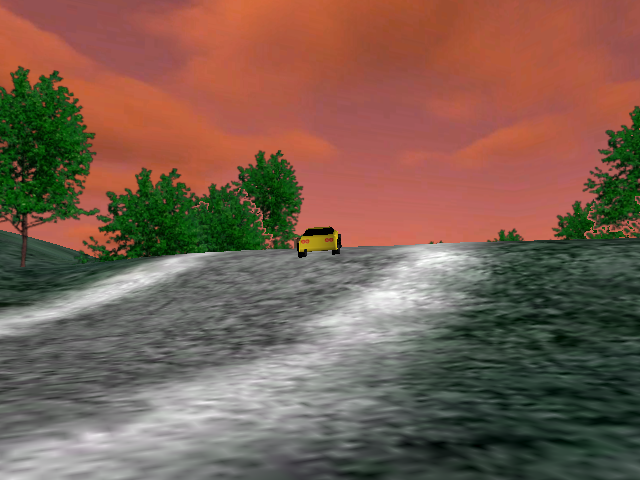
\includegraphics[scale=0.250]{./conluz.png}
 % startinggrid.png: 640x480 pixel, 72dpi, 22.58x16.93 cm, bb=0 0 640 480
 \caption{Juego con todas las luces habilitadas.}
\label{fig:conluz}
\end{minipage}
\end{figure}



\section{Características Extra}
\label{caracteristicas}

Dentro de las características opcionales a implementar, el equipo se inclinó
por las siguientes: texturas procedurales, capturas de pantallas, árboles con
billboards, diferentes skyboxes, c\'amaras est\'aticas y velocimetro.

\subsection{Texturas Procedurales}

Para la realización de las texturas procedurales, el desarrollo fue basado en
el diseñado para la extensión del \textit{Trabajo Práctico Número 2 - Ray
Tracer}.  Se implementaron dos texturas procedurales, piedra y marmol.

\begin{figure}
\begin{minipage}[b]{0.5\linewidth}
\centering
 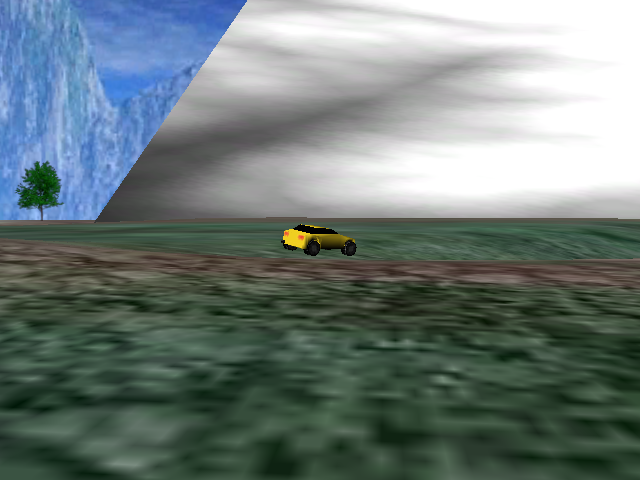
\includegraphics[scale=0.250]{./marble.png}
 % startinggrid.png: 640x480 pixel, 72dpi, 22.58x16.93 cm, bb=0 0 640 480
 \caption{Textura Procedural: Marmol.}
\label{fig:figure5}
\end{minipage}
\hspace{0.5cm}
\begin{minipage}[b]{0.5\linewidth}
\centering
 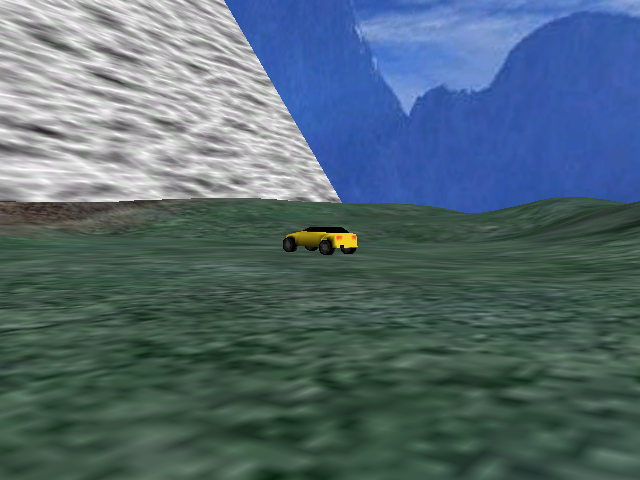
\includegraphics[scale=0.250]{./stone.png}
 % startinggrid.png: 640x480 pixel, 72dpi, 22.58x16.93 cm, bb=0 0 640 480
 \caption{Textura Procedural: Piedra}
\label{fig:figure6}
\end{minipage}
\end{figure}

Donde en la figura \ref{fig:figure5} y \ref{fig:figure6} se puede observar las
dos texturas procedurales realizadas, marmol y piedra respectivamente.

Las dos fueron realizadas utilizando Perlin Noise, realizando las sumas
sucesivas de los ruidos para distintas frecuencias.  Para más detalle,
remitirse al informe del \textit{Trabajo Práctico Número 2 - Extensión}.

\subsection{Capturas de Pantalla}

Otra de las características desarrolladas, fue la posibilidad de obtener
capturas de pantallas de cualquier momento del juego.  Para realizar dicha
acción, hay que presionar la tecla ``0`` (cero) en cualquier momento del
mismo.

Las imágenes producidas, son almacenadas en la raíz del proyecto, y el nombre
con el que se guardan es la fecha en que fueron realizados.

Esta característica fue muy utilizada a la hora de realizar este informe.

\subsection{Billboards}

Otra característica implementada, fue el hecho de contar con árboles
realizados
con texturas de tipo billboard.

En las imágenes presentadas con antelación y más precisamente en la figura
\ref{fig:figure7}, puede observarse cómo este tipo de árboles son utilizados a
lo largo de todo el recorrido; donde también cabe mencionar que el vehículo
puede colisionar contra este tipo de texturas.

Algo interesante sobre este tipo de texturas es que nos brindan la posibilidad
de verlas correctamente desde cualquier ángulo, además permitiendo que se vean
con claridad las otras texturas detras de ellas.

\begin{figure}
 \centering
 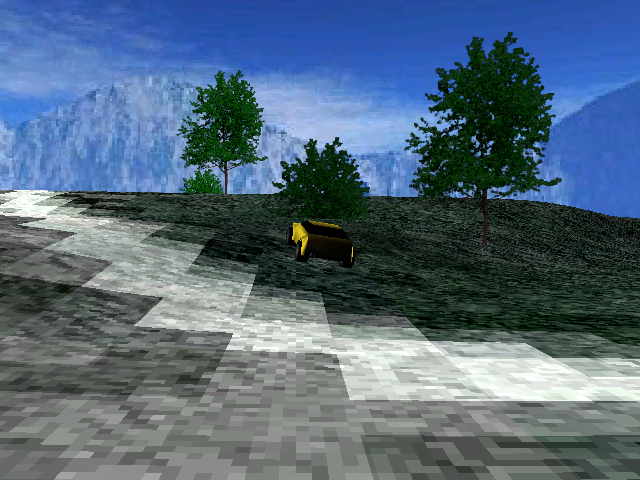
\includegraphics[scale=0.4]{./billboard.png}
 % billboard.png: 640x480 pixel, 72dpi, 22.58x16.93 cm, bb=0 0 640 480
 \caption{Árboles con Texturas Billboard.}
 \label{fig:figure7}
\end{figure}


\subsection{Uso y Selecci\'on de distintos \textit{Skyboxes}}

Uno de los opcionales seleccionados para el desarrollo del juego, fue darle al
usuario la posibilidad de elegir distintos skyboxes.  Se ofrecen tres, uno para
el d\'ia, otro para la tarde y el \'ultimo para la noche.

Cuando el jugador selecciona la opci\'on de $New Game$, tiene la posibilidad de
seleccionar el momento del d\'ia en que quiere correr la carrera.  Esto se
ver\'a reflejado en la carrera en si, una vez que comience la misma.  En todas
las im\'agenes presentes en el informe, se puede apreciar el skybox que
pertenece al momento \textit{d\'ia} mientras que en la figura \ref{fig:conluz}
se puede apreciar un cielo rojizo, simulando el atardecer.

\subsection{C\'amaras Est\'aticas}

A lo largo de la carrera, el jugador puede presionar la tecla $C$ y esto va a
cambiar la c\'amara desde donde se ve la carrera.  En cada checkpoint hay una
c\'amara est\'atica que est\'a apuntando al mismo.

En la figura \ref{fig:static} se puede apreciar una c\'amara est\'atica en el
segundo checkpoint.

\begin{figure}
 \centering
 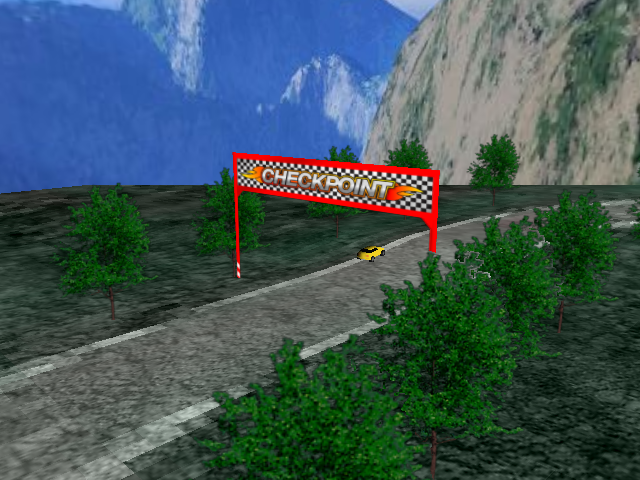
\includegraphics[bb=0 0 640 480,scale=0.4,keepaspectratio=true]{./static.png}
 % static.png: 640x480 pixel, 72dpi, 22.58x16.93 cm, bb=0 0 640 480
 \caption{C\'amara est\'atica en el segundo checkpoint}
 \label{fig:static}
\end{figure}

\subsection{Velocimetro}

El \'ultimo opcional que decidimos implementar, fue el velocimetro con una
aguja.  Para realizar esto, utilizamos una imagen de un velocimetro sin la
aguja, y un cuadrilatero por separado.  Una vez que tuvimos esto, lo
posicionamos en su lugar y luego le aplicamos a la aguja, una rotaci\'on
dependiendo de la velocidad actual de veh\'iculo.

Dependiendo de la velocidad lineal del veh\'iculo, hacemos una traducci\'on de
ese valor lineal a un \'angulo entre $-112.5$ y $112.5$ grados, que nos da la
rotaci\'on de la aguja para un velocimetro que tolera velocidades entre 0 y 160
kilometros por hora.


\section{Modo de Uso}
\label{mododeuso}
En esta sección, comentaremos la forma de jugar al Rally Uribe 100K.  Cabe
destacar que estas instrucciones están basadas en la configuración default del
juego, ya que cabe la posibilidad de modificar las teclas a utilizar.

\subsection{¿Cómo se Juega?}
Para jugar al juego, solo es necesario conocer las teclas para moverse a traves
de la pista.  Lo único necesario es saber con qué teclas avanzar, retroceder,
girar a la izquierda y a la derecha.  Luego, solo es necesario atravesar los
diferentes checkpoints hasta llegar a la meta.

Por defecto, las teclas para mover el vehiculo a traves del terreno son las
flechas hacia arriba para acelerar, hacia abajo para desacelerar y ir hacia
atras, hacia la izquiera para doblar en esa direcci\'on y hacia la derecha para
doblar a la derecha.

Durante el juego, es posible pausar el mismo mediante la tecla $ESC$ y sacar
$screenshots$ con la tecla $0$.

Adem\'as, es posible cambiar la c\'amara con la que se ve el veh\'iculo a otras
c\'amaras est\'aticas mediante la tecla $C$.

\subsection{Los Menúes}
Para movernos a través de los menúes, es necesario utilizar las flechas hacia
arriba, abajo, izquierda, derecha y el enter.  Con las flechas de arriba y
abajo, marcaremos la opción deseada, mientras que con la tecla de enter,
seleccionaremos la misma.

En las opciones del menú que contengan distintas posibilidades de
configuración, ya sea el momento del día en cual vamos a correr, estado del
sonido y demás opciones, es necesario utilizar las flechas hacia la derecha e
izquierda para cambiar la opción.
\section{Configuración}
\label{configuracion}
El juego, como mencionamos con antelación, tiene ciertas características que
son configurables.  Desde las teclas, las texturas de los skyboxes, las
características de las pistas y las pistas en sí son configurables.

Todas estas características configurables, pueden ser modificadas desde el
archivo "global.properties".

\subsection{Configuración del Juego}

Desde el archivo previamente mencionado, es posible configurar todas las teclas
del juego además de los nombres y texturas de los skyboxes, el estado de la
música y los efectos como las pistas a escucharse ante cada evento y/o pistas
de la música ambiental.  Además, tanto para la música como para los efectos,
es
posible configurar en qué nivel quiere uno que se encuentren, del 0 al 100,
siendo 100 el volumen más alto de la música o efecto.

\subsection{Configuración de Nuevas Pistas}

Desde el archivo de configuración, es posible determinar la posición de los
distintos objetos que componen a la escena.

Los árboles, checkpoints, pirámides con texturas procedurales, como el resto
de
los objetos presentes, pueden ser configurados fácilmente desde el archivo de
configuración.

Para configurar los árboles presentes en la escena, es necesario indicar qué
cantidad de árboles habrá, y acto seguido, indicar para cada uno de esos
árboles, que posición van a ocupar en el terreno.

Un ejemplo del archivo de configuración para la determinación de la posición
de
los árboles es:

\begin{verbatim}
TRACK1.TREE.COUNT=425
TRACK1.TREE1.POS=672, -846
TRACK1.TREE2.POS=664, -859
TRACK1.TREE3.POS=642, -889
...
TRACK1.TREE425.POS=1642, -1889
\end{verbatim}

Donde se puede observar cómo en la primera línea, se le indica la cantidad de
árboles presentes en la escena y luego, para cada uno de los árboles, una
posición dada por dos puntos.

Para el caso de los checkpoints, es similar a los árboles pero con una pequeña
variación, dada por la necesidad de determinar la rotación del plano que
contiene al checkpoint.

Un ejemplo del archivo de configuración para la determinación de la posición
de
los checkpoints es:

\begin{verbatim}
TRACK1.CHECKPOINT.COUNT=8
TRACK1.CHECKPOINT1.POS=515,-806
TRACK1.CHECKPOINT1.ROT=6.68925
TRACK1.CHECKPOINT2.POS=-4434,-3150
TRACK1.CHECKPOINT2.ROT=6.32625
TRACK1.CHECKPOINT3.POS=694,-4591
TRACK1.CHECKPOINT3.ROT=4.748
TRACK1.CHECKPOINT4.POS=3880,-3081
TRACK1.CHECKPOINT4.ROT=3.604
TRACK1.CHECKPOINT5.POS=4094,-138
TRACK1.CHECKPOINT5.ROT=3.126
TRACK1.CHECKPOINT6.POS=2069,1334
TRACK1.CHECKPOINT6.ROT=7.718
TRACK1.CHECKPOINT7.POS=-674,4184
TRACK1.CHECKPOINT7.ROT=2.126
TRACK1.CHECKPOINT8.POS=-4363,3862
TRACK1.CHECKPOINT8.ROT=6.451
\end{verbatim}

Donde aca podemos observar como están presentes los 8 checkpoints utilizados en
la pista presentada, donde cada uno tiene su posición y su rotación en
radiantes.

Otra posibilidad sería la de configurar las pirámides con texturas
procedurales.  De forma similar que los ejemplos presentados con antelación, un
ejemplo de una entrada en el archivo de configuración sería:

\begin{verbatim}
TRACK1.PIRAMID.COUNT=2
TRACK1.PIRAMID1.POS=2858,2142
TRACK1.PIRAMID1.TYPE=Marble
TRACK1.PIRAMID2.POS=1850,-150
TRACK1.PIRAMID2.TYPE=Stone
\end{verbatim}

Donde además de indicar la cantidad de pirámides que van a haber en el
terreno,
es necesario indicarle que textura utilizaran.  Previamente en el informe
comentamos la existencia de dos tipos de texturas procedurales, piedra y
marmol, tal como se pueden apreciar en el archivo de configuración de la pista.

Para realizar la pista, el Framework de JME nos provee de una funci\'on para
realizar terrenos.  Uno le indica la altura m\'axima y m\'inima y el terreno es
generado por el Framework.  Para modificar la textura del terreno, utilizamos
una imagen obtenida de Google Maps y modificada para que sea una pista de
carreras.  Hay dos archivos utilizados para la pista, "autodromo2.png" y
"autodromo2low.png".  El primero es la pista con alta nivel de detalle y el
segundo es la pista con un nivel de detalle m\'as bajo.

\section{Conclusión}
\label{conclusiones}

A lo largo del desarrollo del juego, pudimos adquirir varios conceptos y
enseñanzas del proceso que conlleva crear y desarrollar uno.

Para comenzar, adquirimos conocimientos sobre las distintas partes que componen
a un juego, las distintas fases de los mismos y además, logramos adquirir
cierta experiencia utilizando un framework para el desarrollo de videojuegos en
Java.

Cabe destacar que debido a que el grupo eligió utilizar JME2 para el desarrollo
del juego, ante cada problema o situación que requirió de asistencia, logramos
sortear el inconveniente gracias a la extensa documentación sobre el Framework
que está disponible en los distintos foros y en la misma documentación propia
de los desarrolladores del mismo.

\end{document}
